\documentclass{beamer}
\usetheme{Madrid}
\usecolortheme{default}
\usepackage{tikz}
\usepackage{amsmath}
\usepackage{amssymb}

\title{Inductive Generalizations: From Patterns to Principles}
\subtitle{Introduction to Logic}
\author{Professor's Name}
\institute{University Name}
\date{\today}

\begin{document}

\begin{frame}
\titlepage
\end{frame}

\begin{frame}
\frametitle{1. Introduction: Reasoning Beyond Deduction}
\begin{itemize}
\item Logic encompasses multiple forms of reasoning that extend beyond simple deduction.
\item Inductive reasoning allows us to make probable inferences about the unknown based on what we observe.
\item These inferences guide our daily decisions and form the backbone of scientific inquiry.
\item Understanding inductive logic helps us evaluate the strength of arguments in everyday life.
\end{itemize}

\begin{block}{Course Goals}
To develop skills for identifying, constructing, and evaluating inductive arguments while recognizing their limitations and potential pitfalls.
\end{block}
\end{frame}

\begin{frame}
\frametitle{2. What is Inductive Reasoning?}
\begin{itemize}
\item \textbf{Inductive reasoning} is the process of deriving general principles from specific observations.
\item Unlike deductive reasoning, inductive conclusions are probable rather than certain.
\item The strength of inductive arguments depends on the quality and quantity of evidence.
\item Inductive reasoning is essential in science, medicine, policy-making, and everyday decision-making.
\end{itemize}

\begin{example}
Observation: Every crow I have ever seen is black.\\
Inductive conclusion: All crows are probably black.
\end{example}
\end{frame}

\begin{frame}
\frametitle{3. Deductive vs. Inductive Arguments: Key Differences}
\begin{itemize}
\item \textbf{Deductive arguments} move from general premises to specific conclusions with certainty.
\item \textbf{Inductive arguments} move from specific observations to general conclusions with probability.
\item Deductive arguments are either valid or invalid; inductive arguments are strong or weak.
\item The conclusion of a valid deductive argument must be true if all premises are true.
\end{itemize}

\begin{center}
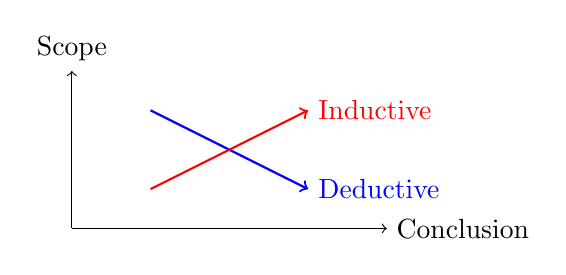
\begin{tikzpicture}
\draw[->] (0,0) -- (4,0) node[right] {Conclusion};
\draw[->] (0,0) -- (0,2) node[above] {Scope};

% Deductive
\draw[thick, blue, ->] (1,1.5) -- (3,0.5) node[right, blue] {Deductive};

% Inductive
\draw[thick, red, ->] (1,0.5) -- (3,1.5) node[right, red] {Inductive};
\end{tikzpicture}
\end{center}
\end{frame}

\begin{frame}
\frametitle{4. The Structure of Inductive Generalizations}
\begin{itemize}
\item Inductive generalizations move from observed instances to claims about all instances of a similar type.
\item The basic form is: "Most observed Xs have property Y, therefore all (or most) Xs probably have property Y."
\item The premises include observations about a sample of a population.
\item The conclusion extends what was observed in the sample to the entire population.
\end{itemize}

\begin{alertblock}{Important Note}
The relationship between sample and population is critical to the strength of an inductive generalization.
\end{alertblock}
\end{frame}

\begin{frame}
\frametitle{5. Strong vs. Weak Inductive Arguments}
\begin{itemize}
\item A \textbf{strong inductive argument} provides good grounds for accepting its conclusion as probable.
\item A \textbf{weak inductive argument} fails to provide sufficient support for its conclusion.
\item The strength of an inductive argument depends on the quality and quantity of evidence.
\item Even strong inductive arguments can lead to false conclusions.
\end{itemize}

\begin{columns}
\column{0.5\textwidth}
\textbf{Strong:}\\
95\% of 1,000 randomly selected voters prefer Candidate A.\\
Therefore, Candidate A will likely win the election.

\column{0.5\textwidth}
\textbf{Weak:}\\
My three friends prefer Candidate B.\\
Therefore, Candidate B will likely win the election.
\end{columns}
\end{frame}

\begin{frame}
\frametitle{6. Sample Size: Why It Matters}
\begin{itemize}
\item \textbf{Sample size} refers to the number of observations or instances examined in an inductive argument.
\item Larger sample sizes generally provide stronger support for inductive conclusions.
\item Small samples are more vulnerable to random variation and outliers.
\item The law of large numbers states that as sample size increases, sample statistics approach population parameters.
\end{itemize}

\begin{block}{The Relationship Between Sample Size and Confidence}
As sample size increases, our confidence in generalizations increases, but never reaches absolute certainty.
\end{block}
\end{frame}

\begin{frame}
    \frametitle{Case Study: SpongeBob's Hasty Generalization}
    
    \begin{itemize}
    \item \textbf{Character:} SpongeBob SquarePants
    \item \textbf{Scenario:} In "Ripped Pants," SpongeBob accidentally rips his pants at the beach and gets laughs
    \item \textbf{Hasty conclusion:} "Ripping my pants always makes people laugh"
    \item \textbf{Action:} SpongeBob repeatedly rips his pants in different situations
    \item \textbf{Result:} Everyone becomes annoyed rather than amused
    \end{itemize}
    
    \begin{alertblock}{Why This Is Flawed Induction}
    SpongeBob generalized from a single instance, ignoring context and the law of diminishing returns. He failed to consider that situational humor often depends on novelty and surprise.
    \end{alertblock}
    \end{frame}

\begin{frame}
\frametitle{7. Representative Samples: Quality Over Quantity}
\begin{itemize}
\item A \textbf{representative sample} accurately reflects the relevant characteristics of the population being studied.
\item Size alone does not guarantee representativeness—sample composition is equally important.
\item Non-representative samples lead to inaccurate generalizations regardless of sample size.
\item Representative samples control for variables that might affect the property being studied.
\end{itemize}

\begin{example}
Sampling only college students for a study on political attitudes would not be representative of the general population, even with thousands of participants.
\end{example}
\end{frame}

\begin{frame}
\frametitle{8. Random Sampling: Eliminating Bias}
\begin{itemize}
\item \textbf{Random sampling} means every member of a population has an equal chance of being selected.
\item Random sampling helps minimize selection bias in inductive generalizations.
\item Systematic, convenience, and voluntary response sampling methods can introduce bias.
\item Stratified random sampling ensures representation across important subgroups.
\end{itemize}

\begin{alertblock}{Warning}
Even with random sampling, chance variations can create unrepresentative samples, especially with small sample sizes.
\end{alertblock}
\end{frame}

\begin{frame}
\frametitle{9. Basic Statistical Concepts: Mean, Median, Mode}
\begin{itemize}
\item \textbf{Mean} is the arithmetic average of all values in a dataset (sum divided by count).
\item \textbf{Median} is the middle value when data is arranged in order (less affected by outliers).
\item \textbf{Mode} is the most frequently occurring value in a dataset.
\item These measures of central tendency help summarize data for inductive reasoning.
\end{itemize}

\begin{table}
\centering
\begin{tabular}{|l|c|c|c|}
\hline
\textbf{Dataset} & \textbf{Mean} & \textbf{Median} & \textbf{Mode} \\
\hline
[2,2,3,4,5,9] & 4.2 & 3.5 & 2 \\
\hline
[3,3,4,4,4,5,6] & 4.1 & 4 & 4 \\
\hline
\end{tabular}
\caption{Comparing measures of central tendency}
\end{table}
\end{frame}

\begin{frame}
\frametitle{10. Measures of Dispersion: Range, Variance, Standard Deviation}
\begin{itemize}
\item \textbf{Range} is the difference between the maximum and minimum values in a dataset.
\item \textbf{Variance} measures how far individual values spread from the mean.
\item \textbf{Standard deviation} is the square root of variance, indicating typical deviation from the mean.
\item Dispersion measures help assess the reliability of inductive generalizations.
\end{itemize}

\begin{example}
Two classes both have a mean score of 80, but Class A has a standard deviation of 5 while Class B has a standard deviation of 15. Class A's performance is more consistent, making generalizations about performance more reliable.
\end{example}
\end{frame}


\begin{frame}
    \frametitle{Case Study: Lisa Simpson's Representative Sample}
    
    \begin{itemize}
    \item \textbf{Character:} Lisa Simpson (The Simpsons)
    \item \textbf{Research question:} Is a new educational toy effective?
    \item \textbf{Methodology:} Selects diverse students across different grades, abilities, and backgrounds
    \item \textbf{Data collection:} Before, during, and after toy use over several weeks
    \item \textbf{Analysis:} Controls for variables and considers statistical significance
    \end{itemize}
    
    \begin{block}{Why This Is Strong Induction}
    Lisa creates a representative sample that reflects the broader student population, controls for confounding variables, and collects sufficient longitudinal data before making her generalization.
    \end{block}
    \end{frame}

\begin{frame}
\frametitle{11. Correlation vs. Causation: A Critical Distinction}
\begin{itemize}
\item \textbf{Correlation} occurs when two variables change together in a systematic way.
\item \textbf{Causation} means changes in one variable directly cause changes in another.
\item Correlation does not necessarily imply causation.
\item Alternative explanations for correlation include: reverse causation, common cause, coincidence, and confounding variables.
\end{itemize}

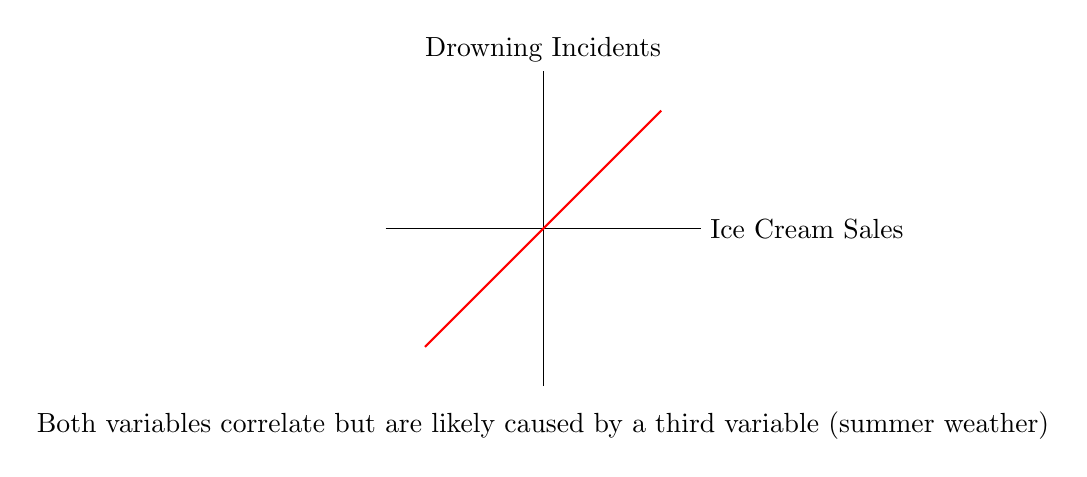
\begin{tikzpicture}
\draw (-2,0) -- (2,0) node[right] {Ice Cream Sales};
\draw (0,-2) -- (0,2) node[above] {Drowning Incidents};
\draw[red, thick] (-1.5,-1.5) -- (1.5,1.5);
\node at (0,-2.5) {Both variables correlate but are likely caused by a third variable (summer weather)};
\end{tikzpicture}
\end{frame}


\begin{frame}
\frametitle{12. Statistical Significance: What Does It Mean?}
\begin{itemize}
\item \textbf{Statistical significance} indicates that an observed result is unlikely due to chance alone.
\item Results are typically considered significant when the p-value is less than 0.05 (5\%).
\item A significant result does not necessarily mean the effect is large or important.
\item Statistical significance helps determine whether patterns observed in samples reflect actual population trends.
\end{itemize}

\begin{alertblock}{Common Misconception}
Statistical significance does not tell us the probability that the hypothesis is true, only the probability of seeing the observed results if the null hypothesis were true.
\end{alertblock}
\end{frame}

\begin{frame}
\frametitle{13. Confidence Intervals: Expressing Uncertainty}
\begin{itemize}
\item A \textbf{confidence interval} is a range of values likely to contain the true population parameter.
\item A 95\% confidence interval means that if we repeated the sampling procedure many times, 95\% of intervals would contain the true value.
\item Wider intervals indicate greater uncertainty about the population parameter.
\item Confidence intervals provide more information than simple point estimates.
\end{itemize}

\begin{center}
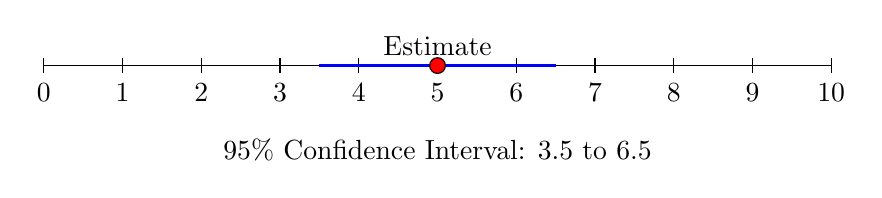
\begin{tikzpicture}
\draw[-] (0,0) -- (10,0);
\foreach \x in {0,1,2,3,4,5,6,7,8,9,10}
\draw (\x,0.1) -- (\x,-0.1) node[below] {\x};
\draw[thick, blue] (3.5,0) -- (6.5,0);
\draw[fill=red] (5,0) circle (0.1) node[above] {Estimate};
\node[below] at (5,-0.8) {95\% Confidence Interval: 3.5 to 6.5};
\end{tikzpicture}
\end{center}
\end{frame}

\begin{frame}
\frametitle{14. The Problem of Induction: Hume's Challenge}
\begin{itemize}
\item Philosopher David Hume questioned whether inductive reasoning can ever be rationally justified.
\item The \textbf{problem of induction} points out that we cannot prove future observations will resemble past ones.
\item Any attempt to justify induction with past success uses inductive reasoning itself, creating circular logic.
\item Despite this philosophical challenge, inductive reasoning remains practically indispensable.
\end{itemize}

\begin{block}{Hume's Classic Example}
The sun has risen every day in recorded history. We infer it will rise tomorrow, but cannot deductively prove this—we rely on the assumption that nature is uniform.
\end{block}
\end{frame}

\begin{frame}
\frametitle{15. Enumerative Induction: From Specifics to Generals}
\begin{itemize}
\item \textbf{Enumerative induction} reasons from observed instances to a general conclusion about all similar instances.
\item The form is: "X\textsubscript{1} has property P, X\textsubscript{2} has property P, ..., therefore all Xs probably have property P."
\item Strength depends on number of observations, variety of circumstances, and absence of counterexamples.
\item This is the most basic form of inductive generalization.
\end{itemize}

\begin{example}
Observed: Swan 1 is white. Swan 2 is white. Swan 3 is white...\\
Conclusion: All swans are probably white.\\
(This was believed until black swans were discovered in Australia.)
\end{example}
\end{frame}


\begin{frame}
\frametitle{16. Statistical Syllogisms: From Generals to Specifics}
\begin{itemize}
\item A \textbf{statistical syllogism} moves from a general probability to a specific instance.
\item The form is: "X\% of Fs are Gs, object O is an F, therefore O is probably a G."
\item The strength depends on the percentage X and whether O is a typical F.
\item Statistical syllogisms are the reverse of enumerative induction.
\end{itemize}

\begin{alertblock}{Important Distinction}
Unlike enumerative induction (moving from specifics to generals), statistical syllogisms move from generals to specifics—from populations to individuals.
\end{alertblock}
\end{frame}

\begin{frame}
\frametitle{17. Inferences to the Best Explanation}
\begin{itemize}
\item \textbf{Inference to the best explanation (IBE)} selects the hypothesis that best explains the available evidence.
\item IBE evaluates competing explanations based on simplicity, scope, consistency, and explanatory power.
\item This form of reasoning is common in science, history, medicine, and detective work.
\item IBE is more sophisticated than simple enumerative induction.
\end{itemize}

\begin{columns}
\column{0.45\textwidth}
\textbf{Observed:}
\begin{itemize}
\item Wet ground
\item Water puddles
\item Dark clouds
\end{itemize}

\column{0.55\textwidth}
\textbf{Best explanation:}
It rained recently (better than alternatives like "someone sprayed water everywhere" or "dew formed overnight")
\end{columns}
\end{frame}

\begin{frame}
\frametitle{18. Case Study: Scientific Method as Inductive Reasoning}
\begin{itemize}
\item The scientific method relies heavily on inductive reasoning to develop theories from observations.
\item Scientists observe patterns, formulate hypotheses, test predictions, and refine theories inductively.
\item Scientific knowledge is considered provisional and subject to revision with new evidence.
\item The success of science demonstrates the practical value of inductive reasoning despite its philosophical limitations.
\end{itemize}

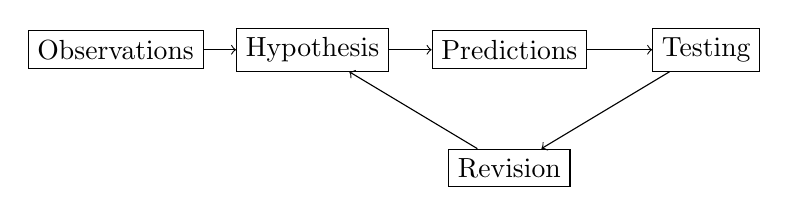
\begin{tikzpicture}[node distance=1.5cm]
\node (obs) [draw, rectangle] {Observations};
\node (hyp) [draw, rectangle, right of=obs, xshift=1cm] {Hypothesis};
\node (pred) [draw, rectangle, right of=hyp, xshift=1cm] {Predictions};
\node (test) [draw, rectangle, right of=pred, xshift=1cm] {Testing};
\node (rev) [draw, rectangle, below of=pred] {Revision};

\draw[->] (obs) -- (hyp);
\draw[->] (hyp) -- (pred);
\draw[->] (pred) -- (test);
\draw[->] (test) -- (rev);
\draw[->] (rev) -- (hyp);
\end{tikzpicture}
\end{frame}

\begin{frame}
\frametitle{19. Common Fallacy: Hasty Generalization}
\begin{itemize}
\item A \textbf{hasty generalization} draws a conclusion based on insufficient evidence or too small a sample.
\item This fallacy results in generalizations that go beyond what the evidence actually supports.
\item It often arises from our tendency to see patterns even with limited data.
\item Hasty generalizations lead to stereotypes and prejudices when applied to social groups.
\end{itemize}

\begin{example}
"I met two rude people from Chicago, so people from Chicago must be rude."

This generalizes from just two instances to an entire population of millions, making it a hasty generalization.
\end{example}
\end{frame}


\begin{frame}
\frametitle{20. Common Fallacy: Biased Samples}
\begin{itemize}
\item A \textbf{biased sample} is not representative of the population it's meant to describe.
\item Types of bias include selection bias, voluntary response bias, and convenience sampling.
\item Biased samples systematically exclude or over-represent certain segments of the population.
\item Generalizations based on biased samples lead to flawed conclusions even with large samples.
\end{itemize}

\begin{alertblock}{Historical Example}
The 1936 Literary Digest poll predicted Alf Landon would defeat Franklin Roosevelt in a landslide. The sample was biased toward wealthy Americans (who owned telephones and magazine subscriptions), producing a severely flawed prediction.
\end{alertblock}
\end{frame}

\begin{frame}
\frametitle{21. Common Fallacy: Post Hoc Ergo Propter Hoc}
\begin{itemize}
\item \textbf{Post hoc ergo propter hoc} ("after this, therefore because of this") mistakenly assumes that if B follows A, then A caused B.
\item This fallacy confuses temporal sequence with causation.
\item It ignores other potential causes, coincidence, or underlying factors.
\item This fallacy is common in everyday reasoning, superstitions, and pseudoscience.
\end{itemize}

\begin{example}
"I wore my lucky socks and our team won the game, so my socks caused our victory."

The temporal sequence exists, but there's no causal connection between the socks and the team's performance.
\end{example}
\end{frame}

\begin{frame}
\frametitle{22. Common Fallacy: Ecological Fallacy}
\begin{itemize}
\item The \textbf{ecological fallacy} occurs when inferences about individuals are drawn from data about groups.
\item It improperly assumes that group-level characteristics apply to all members of that group.
\item Group averages can mask significant individual variation within the group.
\item This fallacy often appears in discussions of demographic data and social statistics.
\end{itemize}

\begin{columns}
\column{0.5\textwidth}
\textbf{Group-level data:}
State A has a higher average income than State B.

\column{0.5\textwidth}
\textbf{Ecological fallacy:}
Any person from State A will be wealthier than any person from State B.
\end{columns}
\end{frame}

\begin{frame}
\frametitle{23. Common Fallacy: Texas Sharpshooter}
\begin{itemize}
\item The \textbf{Texas Sharpshooter Fallacy} involves cherry-picking data clusters to suit a pre-determined conclusion.
\item Named after a hypothetical shooter who fires at a barn then draws targets around the bullet holes.
\item This fallacy ignores the random distribution of data and focuses only on apparent patterns.
\item It commonly appears in claims about cancer clusters, economic predictions, and conspiracy theories.
\end{itemize}

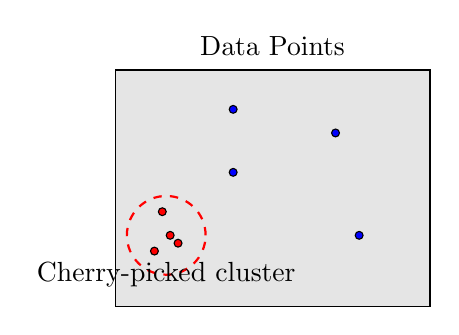
\begin{tikzpicture}
\draw[fill=gray!20] (0,0) rectangle (4,3);
\node at (2,3.3) {Data Points};
\draw[fill=red] (0.5,0.7) circle (0.05);
\draw[fill=red] (0.7,0.9) circle (0.05);
\draw[fill=red] (0.6,1.2) circle (0.05);
\draw[fill=red] (0.8,0.8) circle (0.05);
\draw[fill=blue] (1.5,1.7) circle (0.05);
\draw[fill=blue] (3.1,0.9) circle (0.05);
\draw[fill=blue] (1.5,2.5) circle (0.05);
\draw[fill=blue] (2.8,2.2) circle (0.05);
\draw[red, thick, dashed] (0.65,0.9) circle (0.5);
\node at (0.65,0.4) {Cherry-picked cluster};
\end{tikzpicture}
\end{frame}

\begin{frame}
\frametitle{24. Cognitive Bias: Confirmation Bias}
\begin{itemize}
\item \textbf{Confirmation bias} is the tendency to search for, interpret, and recall information that confirms existing beliefs.
\item This bias leads us to give greater weight to evidence supporting our views and dismiss contradicting evidence.
\item Confirmation bias affects which data we collect and how we interpret ambiguous information.
\item This bias can strengthen beliefs even when they contradict objective evidence.
\end{itemize}

\begin{block}{Overcoming Confirmation Bias}
To counter confirmation bias, actively seek disconfirming evidence, consider alternative hypotheses, and invite critical feedback from others with different perspectives.
\end{block}
\end{frame}

\begin{frame}
    \frametitle{Case Study: Squidward's Confirmation Bias}
    
    \begin{itemize}
    \item \textbf{Character:} Squidward Tentacles (SpongeBob SquarePants)
    \item \textbf{Belief:} "SpongeBob is always annoying and never helpful"
    \item \textbf{Evidence filtering:} Remembers and dwells on every time SpongeBob disrupts his clarinet practice
    \item \textbf{Selective memory:} Ignores or downplays the many times SpongeBob has helped him
    \item \textbf{Reinforcement:} Only notices SpongeBob's irritating traits, never his positive qualities
    \end{itemize}
    
    \begin{alertblock}{Why This Is Flawed Induction}
    Squidward selectively focuses on evidence that confirms his negative view while dismissing contradictory evidence, similar to how people form persistent biases about coworkers, neighbors, or family members.
    \end{alertblock}
    \end{frame}

\begin{frame}
\frametitle{25. Cognitive Bias: Availability Heuristic}
\begin{itemize}
\item The \textbf{availability heuristic} leads us to judge probability based on how easily examples come to mind.
\item Vivid, recent, or emotionally charged events are more "available" in memory and seem more common.
\item This heuristic can distort risk assessment and lead to irrational fears.
\item Media coverage often amplifies the availability heuristic by highlighting rare but dramatic events.
\end{itemize}

\begin{example}
After hearing news reports about shark attacks, people often overestimate their likelihood. In reality, the annual risk of death from a shark attack is approximately 1 in 3.7 million, far less than everyday risks like driving.
\end{example}
\end{frame}

\begin{frame}
    \frametitle{Case Study: Sokka's Availability Heuristic}
    
    \begin{itemize}
    \item \textbf{Character:} Sokka (Avatar: The Last Airbender)
    \item \textbf{Experience:} After narrowly escaping an angry platypus bear, Sokka becomes overly cautious about wildlife
    \item \textbf{Flawed reasoning:} "Wild animals are extremely dangerous and attack people constantly!"
    \item \textbf{Evidence:} Bases his fear on one vivid, emotionally charged experience
    \item \textbf{Reality:} Most wildlife encounters are peaceful, and attacks are statistically rare
    \end{itemize}
    
    \begin{alertblock}{Why This Is Flawed Induction}
    Sokka overestimates the frequency of animal attacks based on how easily he can recall one frightening example, similar to how people overestimate risks of plane crashes, shark attacks, or crime after exposure to dramatic news stories.
    \end{alertblock}
    \end{frame}

\begin{frame}
\frametitle{26. Cognitive Bias: Representativeness Heuristic}
\begin{itemize}
\item The \textbf{representativeness heuristic} judges probability by how well something matches our mental prototype.
\item We tend to ignore base rates and focus on how typical or representative a case seems.
\item This heuristic leads to errors when appearances are misleading or stereotypical.
\item It can result in overlooking statistical information in favor of narrative coherence.
\end{itemize}

\begin{alertblock}{Classic Example}
Consider "Linda is 31, single, outspoken, and very bright. She majored in philosophy. As a student, she was deeply concerned with discrimination and social justice issues."

People often rate "Linda is a bank teller and active in the feminist movement" as more probable than "Linda is a bank teller," violating basic probability (conjunction fallacy).
\end{alertblock}
\end{frame}

\begin{frame}
\frametitle{27. Cognitive Bias: Base Rate Fallacy}
\begin{itemize}
\item The \textbf{base rate fallacy} occurs when we ignore the background statistical frequency of an event.
\item We focus on specific information about a case and neglect relevant general probabilities.
\item This fallacy is closely related to the representativeness heuristic.
\item It commonly appears in medical diagnoses, criminal profiling, and risk assessment.
\end{itemize}

\begin{table}
\centering
\begin{tabular}{|l|c|c|}
\hline
\textbf{Test Result} & \textbf{Has Disease} & \textbf{No Disease} \\
\hline
Positive & 99 (True +) & 999 (False +) \\
\hline
Negative & 1 (False -) & 8,901 (True -) \\
\hline
\end{tabular}
\caption{For a disease with 1\% prevalence and a 99\% accurate test, a positive result only indicates a 9\% chance of disease due to base rates}
\end{table}
\end{frame}

\begin{frame}
\frametitle{28. Cognitive Bias: Anchoring Effect}
\begin{itemize}
\item The \textbf{anchoring effect} is the tendency to rely too heavily on the first piece of information encountered.
\item Initial values "anchor" subsequent judgments even when the anchor is arbitrary or irrelevant.
\item This bias affects numerical estimates, negotiations, and decision-making.
\item Anchoring persists even when people are aware of the bias and try to avoid it.
\end{itemize}

\begin{example}
In a classic study, people spun a wheel rigged to stop at either 10 or 65, then estimated the percentage of African countries in the UN. Those who saw "10" guessed 25\% on average, while those who saw "65" guessed 45\% on average.
\end{example}
\end{frame}

\begin{frame}
\frametitle{29. Real-World Applications: Opinion Polls}
\begin{itemize}
\item Opinion polls apply inductive reasoning to estimate public attitudes from sample responses.
\item The accuracy of polls depends on sample size, randomization, and question wording.
\item \textbf{Margin of error} represents the range within which the true population value likely falls.
\item Common polling issues include selection bias, response bias, and question order effects.
\end{itemize}

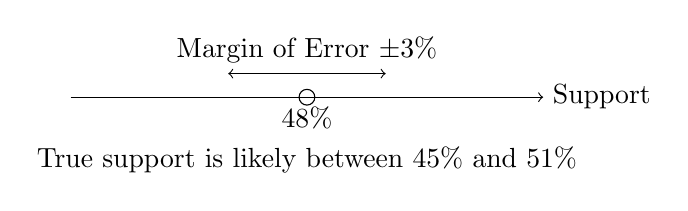
\begin{tikzpicture}
\draw[->] (0,0) -- (6,0) node[right] {Support};
\draw (3,0) circle (0.1) node[below] {48\%};
\draw[<->] (2,0.3) -- (4,0.3);
\node at (3,0.6) {Margin of Error $\pm$3\%};
\node at (3,-0.8) {True support is likely between 45\% and 51\%};
\end{tikzpicture}
\end{frame}

\begin{frame}
\frametitle{30. Real-World Applications: Medical Testing}
\begin{itemize}
\item Medical diagnoses rely on inductive reasoning from test results to health conclusions.
\item \textbf{Sensitivity} is the probability of a positive test result if the disease is present.
\item \textbf{Specificity} is the probability of a negative test result if the disease is absent.
\item The base rate of a disease strongly affects the predictive value of test results.
\end{itemize}

\begin{block}{Bayes' Theorem in Practice}
The probability of having a disease given a positive test depends on the test's accuracy and the disease prevalence. For rare diseases, even highly accurate tests can yield many false positives.
\end{block}
\end{frame}

\begin{frame}
\frametitle{31. Real-World Applications: Legal Reasoning}
\begin{itemize}
\item Legal reasoning often uses inductive arguments to establish facts beyond reasonable doubt.
\item Evidence is evaluated based on relevance, reliability, and probative value.
\item The standard of proof varies by context: "preponderance of evidence" in civil cases versus "beyond reasonable doubt" in criminal cases.
\item Legal systems must balance between Type I errors (convicting the innocent) and Type II errors (acquitting the guilty).
\end{itemize}

\begin{columns}
\column{0.5\textwidth}
\textbf{Deductive element:}
Applying established laws and precedents to specific cases

\column{0.5\textwidth}
\textbf{Inductive element:}
Determining facts from evidence and witness testimony
\end{columns}
\end{frame}

\begin{frame}
\frametitle{32. Critical Thinking: Evaluating Media Claims}
\begin{itemize}
    \item Media reports often present statistical claims without sufficient context or methodology.
    \item Critical evaluation requires identifying the source, sample size, and selection methods.
    \item Watch for misleading graphs, cherry-picked data, and correlation-causation confusion.
    \item Claims that seem surprising or confirm partisan narratives deserve extra scrutiny.
\end{itemize}

\begin{alertblock}{Questions to Ask About Statistical Claims}
\begin{itemize}
    \item Who conducted the research and might they be biased?
    \item How large and representative was the sample?
    \item Are important details or limitations being omitted?
    \item Does the conclusion actually follow from the data presented?
\end{itemize}
\end{alertblock}
\end{frame}

\begin{frame}
\frametitle{33. Critical Thinking: Reading Research Studies}
\begin{itemize}
    \item Scientific research papers provide the most detailed look at how inductive conclusions are drawn.
    \item The methods section describes sampling, measurements, and procedures.
    \item The results section presents data without interpretive claims.
    \item The discussion section offers interpretations but should acknowledge limitations.
\end{itemize}

\begin{block}{Red Flags in Research}
Look for small sample sizes, convenience samples, conflicting interests, unreplicated results, and conclusions that go beyond what the data actually shows.
\end{block}
\end{frame}

\begin{frame}
\frametitle{34. Special Topic: Bayesian Reasoning}
\begin{itemize}
    \item \textbf{Bayesian reasoning} updates probability estimates as new evidence becomes available.
    \item It begins with a prior probability and revises it based on new information.
    \item The formula combines the prior probability with the likelihood of evidence given competing hypotheses.
    \item Bayesian reasoning formalizes how rational beliefs should change with evidence.
\end{itemize}

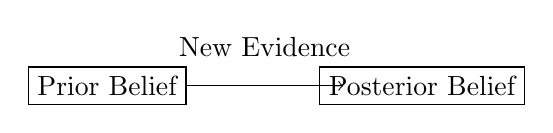
\begin{tikzpicture}
\node[draw] at (0,0) {Prior Belief};
\node[draw] at (4,0) {Posterior Belief};
\draw[->] (1,0) -- (3,0);
\node at (2,0.5) {New Evidence};
\end{tikzpicture}
\end{frame}

\begin{frame}
\frametitle{35. Improving Your Inductive Reasoning Skills}
\begin{itemize}
    \item Seek diverse and representative evidence before drawing general conclusions.
    \item Consider base rates and prior probabilities when evaluating new information.
    \item Actively look for counterexamples to test the strength of generalizations.
    \item Remain open to revising beliefs when confronted with contradictory evidence.
\end{itemize}

\begin{example}
Instead of concluding "This restaurant is excellent" after one good meal (hasty generalization), visit several times, try different menu items, and go at different times of day to gather more representative evidence.
\end{example}
\end{frame}

\begin{frame}
\frametitle{36. Conclusion: Balancing Skepticism and Inference}
\begin{itemize}
    \item Inductive reasoning is essential but inherently probabilistic and fallible.
    \item Critical thinking requires balancing healthy skepticism with practical inference.
    \item Understanding common fallacies and biases helps us avoid reasoning errors.
    \item Strong inductive reasoning acknowledges uncertainty while seeking the most reliable conclusions possible.
\end{itemize}

\begin{block}{Final Thought}
The goal is not perfect certainty (which induction cannot provide) but reasoned judgment that proportions belief to evidence and remains open to revision.
\end{block}
\end{frame}

\end{document}